%
\chapter{Klassenhierarchien}
\label{p:12}
% (rein) virtuelle Methoden -- abstrakte Klassen -- Polymorphismus
% 
% Basisklassenpointer; Nutzung der STL
%
%
%  aus Lectures/advProg/Script/latex: 232 - 1038
%
\section{Ableitungen von Klassen}
\label{sec:A1}
%
%
Dieser Abschnitt der Vorlesung orientiert sich an \cite[\S7]{Microsoft:1993:REC}
und wir beginnen mit den objektorientierten Sprachunterst"utzungen von C++.

Wir stellen uns ein M"obelhaus mit drei Arten von Angestellten vor:
den normalen Angestellten, den Verk"aufern und den Managern.
Von allen ben"otigt die Buchhaltung den Namen, die Lohnverrechnung
ist jedoch unterschiedlich.
So wird der Angestellte (\texttt{Worker}) auf Stundenbasis bezahlt,
der Verk"aufer (\texttt{salesPerson}) auf Stundenbasis  und Verkaufsprovision,
der Manager (\texttt{Manager}) erh"alt ein w"ochentliches Gehalt.

Nat"urlich k"onnte man nun 3 Klassen/Strukturen konventionell programmieren und
dann mit \verb|switch|-Anweisungen immer unterscheiden, welche Variante der Lohnverrechnung
nun benutzt werden soll. Dieses Konzept ist aber sehr fehleranf"allig bzgl. der
Erweiterbarkeit unserer Angstelltenklassen (Verkaufsmanager, Aktienindexmanager), da
dann \textbf{immer alle} \verb|switch|-Anweisungen ge"andert werden m"ussen -
und irgendetwas vergi"st man immer.

Der objektorientierte Ansatz stellt erstmal die Frage nach den gemeinsamen
Eigenschaften unserer Angestellten und dann erst nach den Unterschieden.
Die Gemeinsamkeiten bei allen sind der Name und die notwendige Lohnberechnung.
Unterschiede bestehen in der Art und Weise der Lohnberechnung und der daf"ur notwendigen
Daten. Zus"atzlich k"onnte \texttt{salesPerson} die stundenbasierte
Lohnberechnung von \texttt{Worker} nutzen.
%
\subsection{Design einer Klassenhierarchie}
\label{sec:A1.1}
%
Die für die Angestellten des Möbelhauses betrachteten gemeinsamen und zusätzlichen Eigenschaften 
% Diese Betrachtungen stehen in enger Verbindung mit dem Vererbungskonzept im
stehen in enger Verbindung mit dem Vererbungskonzept im
objektorientierten Programmieren.\index{Vererbung}
Dort deklariert man Basisklassen\index{Klasse!Basis-}, von denen weitere Klassen,
mit zus"atzlichen Eigenschaften ableitet\index{Klasse!abgeleitete} werden.
In \cite[\S8.2]{Schmaranz:2002:SCP} ist dieses Vererbungskonzept sehr
sch"on erl"autert:
\begin{itemize}
 \item Eine Ableitung einer Klasse repr"asentiert
 	eine \textbf{IS-A}-Relation.\index{Klasse!IS-A-Relation}
 \item Eine Membervariable repr"asentiert
 	eine \textbf{HAS A}-Relation\index{Klasse!HAS-A-Relation}
\end{itemize}
%
Diese Relationen werden bei der Ableitung einer Klasse~\texttt{B} von der Basisklasse~\texttt{A} folgendermaßen ersichtlich.
Klasse~\texttt{B} ist eine (\textbf{IS-A}) Basisklasse~\texttt{A} mit den zusätzlichen Eigenschaften (\textbf{HAS A}) 
des Members~\verb|_bb| und der Methode~\verb|fkt_b()|.
%
%  Kurs-C/Try_C++11/Vererbung_a
%
\begin{lstlisting}[caption={Ableitung einer Klasse},label=lst:12_a,
basicstyle=\scriptsize,numbers=left, numberstyle=\tiny, stepnumber=2, numbersep=5pt]
class A                 // Basisklasse
{
   public:
      A(const string& name) : _ss(name)  {};
      string GetString() const
         {return _ss;};
      
   private:
      string _ss;
};

class B: public A       // abgeleitete Klasse erbt  a l l e  Methoden/Member von A
{
   public:
      B(const string& name, int b)
         : A(name), _bb(b)  {};  // Aufruf des Konstruktors der Basisklasse

      int fkt_b() const          // zusaetzliche Methode (Eigenschaft)
         {return _bb*_bb;};
    
   private:
      int _bb;                   // zusaetzlicher Member (Eigenschaft)
};

int main()
{
   A ia("Basis");
   B ib("bin abgeleitet",3); // String-Parameter wird an Basisklasse "durchgereicht"
   
   cout << ia.GetString() << endl;
   cout << ib.GetString() << endl; // abgeleitete Klasse benutzt Basisklassenmethode
   
//   cout << ia.fkt_b();           // fkt_b ist  k e i n e   Basisklassenmethode
   cout << ib.fkt_b();
   
   return 0;
}
\end{lstlisting}
In Zeile~31 des Listings~\ref{lst:12_a} ruft die Instanz~\verb|ib| der Klasse~\texttt{B} 
die Funktion \verb|A::GetString() const|, also eine Methode der Basisklasse. Dies ist wegen 
des \verb|public|-Vererbung in Zeile~12 möglich.


%
%
In unserem Falle des Möbelhauses w"aren alle Angestellen erstmal Besch"aftige, d.h.,
wir ben"otigen eine Basisklasse \texttt{Employee}.
Dann k"onnen wir sagen:
\begin{itemize}
 \item \texttt{Employee} \textbf{HAS-A} Name.
 \item \texttt{Worker} \textbf{IS-A}n \texttt{Employee} und
       \texttt{Worker} \textbf{HAS-A} (zus"atzlich)  einen Stundenlohn und
       eine Arbeitszeit.
 \item \texttt{salesPerson} \textbf{IS-A} \texttt{Worker} und
       \texttt{salesPerson} \textbf{HAS-A} (zus"atzlich)   eine Umsatzbeteiligung am
       erbrachten Umsatz.
 \item \texttt{Manager} \textbf{IS-A}n \texttt{Employee} und
       \texttt{Manager} \textbf{HAS-A} Wochengehalt (zus"atzlich).
\end{itemize}
\begin{minipage}{0.45\textwidth}
Dies ergibt folgende Hierarchy von Klassen. \\
Man beachte, da"s wir bis jetzt noch "uberhaupt keine konkrete
Implementierung angesprochen haben. Vielmehr betrachten wir
nur Eigenschaften der zu handhabenden Objekte. Dieses \textbf{Design}
der Klassenhierarchie\index{Hierarchie!Design}
mu"s immer zu Beginn eines OO-Programmes stehen.
Ein gr"undlich erarbeitetes Design erspart zeitraubende und fehleranf"allige
Umstrukturierungen der Klassenhierarchie in einem sp"ateren
Projektstadium.
\end{minipage}
\hfill
\begin{minipage}{0.5\textwidth}
% \input{hier1.pstex_t}
\label{class_hierarchy}
\centerline{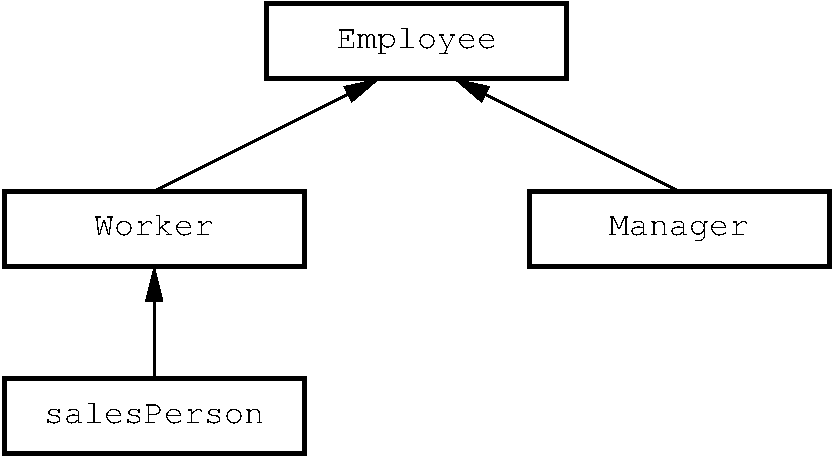
\includegraphics[scale=0.5]{hier1}}
\end{minipage}
%
%
\subsection{Die Basisklasse}
\label{sec:A1.2}
%
Unser Entwurf f"ur die Basisklasse\index{Klasse!Basis-} \texttt{Employee}
sieht folgendermaßen aus:

% \includecode[linerange={4-36,43-46},label=lst:v_9_b_employee]
\includecode[linerange={4-34,42-43,45-45},label=lst:v_9_b_employee]
{v_9b/employee.h}{Basisklasse \texttt{Employee}}

Man beachte, da"s die Methode f"ur die Gehaltsausgabe, \verb|payment()|
in der Basisklasse keine sinnvolle Berechnung ausf"uhren kann, da keinerlei
Daten zur Gehaltsberechnung vorhanden sind. An dieser Stelle kann man wie in Zeile~22 erstmal eine
Dummy-Methode implementieren welche $0.0$ (oder $-12345$) zurückgibt. 
Das Schlüsselwort \index{Methode!virtuelle}\texttt{virtual} weist darauf hin, 
daß diese Methode \emph{virtuell} ist und von abgeleiteten Klassen überladen werden darf.
Deklariert man, wie in Zeile~28 des Listings~\ref{lst:v_9_b_employee}, die Methode 
\verb|payment()| mit dem obskur erscheinenden Konstrukt \verb| = 0 | als \emph{rein virtuelle} Methode,\index{Methode!rein virtuelle} 
dann muß diese Methode in den abgeleiteten Klassen überladen werden, 
siehe~\S\ref{sec:A2}.
%
%
\subsection{Die abgeleiteten Klassen}
\label{sec:A1.3}
%
Unser \texttt{Worker} \textbf{IS-A}n \texttt{Employee} and
\textbf{HAS-A} Stundenlohn und Arbeitszeit.
Diese Zusatzeigenschaften erfordern zusätzliche Methoden
zur ihrer Handhabung und
erlauben nun eine sinnvolle Methode \verb|payment()|.
Gleichzeitig \emph{erbt}\index{Vererbung} \texttt{Employee} alle Eigenschaften von \texttt{Worker}, 
u.a. den Namen und die Zugriffsfunktion darauf.

\includecode[linerange={4-34},label=lst:v_9_b_worker]
{v_9b/worker.h}{abgeleitete Klasse \texttt{Worker}}

Die neuen Eigenschaften (\textbf{HAS-A}) sind in Zeilen~26 und~27 obigen Codefragmentes deklariert.
Zeile~4 beinhaltet die Ableitung der neuen Klasse von der Basisklasse (\textbf{IS-A}).
Das Schl"usselwort \verb|public| in Zeile 4 erlaubt den Zugriff auf Basisklassenmethoden
wie \verb|getname()| "uber Instanzen (Variablen) der Klasse \verb|Worker|.
Dies erlaubt dann folgendes Codefragment:

\begin{lstlisting}[caption={Public Methode der Basisklasse verwenden.},label=lst:ritchie,
basicstyle=\scriptsize,numbers=left, numberstyle=\tiny, stepnumber=2, numbersep=5pt]
  Worker ab("Ritchie Valens");
  cout << ab.getname() << endl;
\end{lstlisting}

Eine Klassenableitung der Form \verb|class Worker : private Employee|
oder \verb|class Worker : protected Employee|
verbietet die Benutzung der Methode \verb|getname()| in obiger Form.
W"ahrend die Verwendung von \verb|protected| wenigstens die Nutzung der Methode
innerhalb der Klasse \verb|Worker| erlaubt, ist selbst dies bei
der Ableitung als \verb|private| nicht m"oglich.

In analoger Weise leiten wir die Klasse \verb|Manager| ab.
%
\includecode[linerange={4-31},label=lst:v_9_b_manager]
{v_9b/manager.h}{abgeleitete Klasse \texttt{Manager}}

Die noch fehlende Klasse \verb|salesPerson| ben"otigt die Klasse \verb|Worker|
als Basisklasse, da die dortige, stundenweise Lohnverrechnung auch hier wieder gebraucht wird.
%
\includecode[linerange={4-38},label=lst:v_9_b_salesperson]
{v_9b/salesperson.h}{abgeleitete Klasse \texttt{salesPerson}}

%
Die Implementierungen s"amtlicher Methoden der vier Klassen sind in den entsprechenden Quelltextfiles und Headerfiles 
zu finden.\bspfile{v_9b.zip}
Hervorzuheben ist an dieser Stelle die Methode
\verb|payment| der Klasse \verb|salesPerson|:
\begin{lstlisting}[caption={Expliziter Aufruf einer Basisklassenmethode.},label=lst:salesPerson::payment,
basicstyle=\scriptsize,numbers=left, numberstyle=\tiny, stepnumber=2, numbersep=5pt]
float salesPerson::payment() const
{
   return Worker::payment() + _commission*_percent;
}
\end{lstlisting}

% \begin{mycode}
% float salesPerson::payment()
% {
%   return Worker::payment() + comission*SalesMade;
% }
% \end{mycode}
Hier ben"otigen wir explizit den Scope-operator \verb|::| um
die \verb|payment|-Methode der Basisklasse \verb|Worker| zu benutzen.
Was w"urde passieren, falls wir  stattdessen
\verb|  return payment() + comission*SalesMade;  | programmieren w"urden?
\index{Scope}

Eine einfache Demonstration unserer neuen Klassen ist in \texttt{v\_9b/main.cpp}\bspfile{v_9b/main.cpp} 
nachzulesen, siehe auch die 
zugehörige \ghref{http://imsc.uni-graz.at/haasegu/Lectures/Kurs-C/Beispiele/v_9b/doxygen/html/class_employee.html}{Dokumentation}.
%
%

%
%
\section{Polymorphismus}
\label{sec:A2}
%
%Der Grund, da"s der Code in \S\ref{sec:A4.3} nicht wie gew"unscht die
Der Grund, da"s der Code \texttt{v\_9b} (ohne Benutzung von \texttt{virtual}) nicht wie gew"unscht die
spezifischen Geh"alter ausgerechnet hat liegt darin, da"s die schon in
der Basisklasse vorhandene Methode \verb|payment()| (und auch \verb|payment()|)
in den abgeleiteten Klassen redefiniert wurde. Dies hat nat"urlich
auf die Basisklasse keine Auswirkung, soda"s eine "uber einen Basisklassenpointer
adressierte Instanz konsequenterweise immer die in der Basisklasse deklarierte Methode
aufruft.

Die Alternative zur Redefinition ist ein Ersatz: Soll eine
Methode der Basisklasse durch eine Methode der abgeleiteten Klasse
\emph{komplett ersetzt} werden, deklariert man diese Methode in der Basisklasse
als \emph{virtuell}\index{virtual}. Das entsprechende Schl"usselwort ist
\verb|virtual|. Ist eine Methode einer Basisklasse virtuell, dann sind
alle gleichnamigen Methoden in abgeleiteten Klassen automatisch virtuell, ohne
da"s das Schl"usselwort angegeben werden mu"s.
%
%
\subsection{Nutzung virtueller Methoden}
\label{sec:A2.1}
%
Mit solchen virtuellen Methoden l"a"st sich erreichen, 
da"s der Code \texttt{v\_9b} so funktioniert, 
%da"s der Code von Seite~\pageref{code:a3_3} so funktioniert, 
da"s immer die richtige
Gehaltsberechnungsmethode in Zeile~38 aufgerufen wird. Dazu m"ussen wir nur
die Basisklasse leicht ab"andern.
% \exfile{A4/employ.hpp}:
\bspfile{A4/employ.hpp}
\begin{lstlisting}[caption={Virtuelle Methoden},label=lst:virt_methode_1,
basicstyle=\scriptsize,numbers=left, numberstyle=\tiny, stepnumber=2, numbersep=5pt]
//			employ.hpp
...
class Employee
{
 public:
  Employee();
  Employee(const string& name);
  const string& getname() const;
  void info();				// Namen ausgeben
  virtual void payment();	//  N E W,  virtuell
  virtual ~Employee()		//  N E W,  jetzt notwendig
  		{};
 private:
  string name;
};
...
\end{lstlisting}

Im Verzeichnis \textit{A4} kann jetzt der Code\bspfile{A4/a4\_1.cpp} mit
\\
\verb|g++ -Wall -o a4_1 a4_1.cpp employ.cpp|
\\
"ubersetzt und gelinkt werden.
%
\pagebreak[2]
\includecode[firstline=13,label=lst:a4_pov]{A4/a4_1.cpp}{Polymorphie ausgenutzt}
%
Die "Anderung in Zeile~10 des Listings~\ref{lst:virt_methode_1} erlaubt es, zur Laufzeit zu entscheiden,
welche Methode \verb| payment() | aufgerufen werden soll.
% \hfill
\\
\begin{minipage}[t]{0.5\textwidth}
In unserem Code bedeutet dies f"ur den letzten Z"ahlzyklus
in den Zeilen 25-28, \\[1ex]
\verb|   for (size_t i=0; i<liste.size(); ++i)| \\
\verb|       { liste[i]->payment(); }| \\[1ex]
da"s folgende Methoden gerufen werden:
\end{minipage}
\hfill
\begin{minipage}[t]{0.45\textwidth}
\begin{tabbing}
 $i=1$ \= \verb| Worker :: payment() | \kill \\
 $i=0$ \> \verb| Employee :: payment() | \\
 $i=1$ \> \verb| Worker :: payment() | \\
 $i=2$ \> \verb| salesPerson :: payment() | \\
 $i=3$ \> \verb| Manager :: payment() | \\
\end{tabbing}
\end{minipage}

Diese M"oglichkeit eine Methode f"ur eine Instanz aufzurufen ohne
dessen Typ genau zu kennen, nennt man \emph{Polymorphie}\index{Polymorphie}.
Dieser griechische Begriff bezeichnet die F"ahigkeit sich von verschiedenen
Seiten zu zeigen oder verschiedene Formen anzunehmen \cite[p.161]{Microsoft:1993:REC}.

Besitzt eine Klasse mind.\  eine virtuelle Methode, dann
mu"s der Destrukor ebenfalls virtuell sein, was in unserer Basisklasse
\verb|Employee| der Fall ist (Der Destruktor ist dort auch gleich definiert.).
Damit man die Notwendigkeit hierf"ur einsieht,\index{Destruktor!virtuell}
betrachten wir das Ende des G"ultigkeitsbereiches von \verb|liste|.
F"ur jedes Element des Arrays von Basisklassenzeigern
wird dann der Destruktor aufgerufen. Ohne einen virtuellen Destruktor in der
Basisklasse w"urde dann stets der Destruktor der Basisklasse aufgerufen.
Dies bewirkt bei abgeleiteten Klassen mit dynamisch allokiertem Speicher, da"s
dieser Speicher nicht freigegeben wird. Bei einem virtuellen
Destruktor der Basisklasse wird wiederum erst zur Laufzeit entscheiden,
welcher Destruktor aufgerufen wird soda"s ein sauberes Speichermanagement
m"oglich ist (es wird erst der Destruktor der abgeleiteten Klasse aufgerufen welcher
seinerseits den Destruktor der Basisklasse implizit aufruft).
%
%
\subsection{Rein virtuelle Methoden}
\label{sec:A2.2}
%
Die Methode \verb|payment()| der Basisklasse \verb|Employee| ist
nur als Platzhalter implementiert und f"uhrt keine sinnvollen Berechnungen aus.
Eigentlich ben"otigen wir diese Methode nur, um anzuzeigen, da"s eine
Methode \verb|payment()| aus abgeleiteten Klassen verwendet werden soll.
Dies ist nicht sonderlich elegant, denn der einzige Zweck von
\verb| Employee :: payment |  besteht darin, \emph{nie} aufgerufen zu werden.

Eine Alternative dazu besteht in einer Methode, die weder semantisch noch
physisch existiert.
Eine derartige Methode ist \emph{rein virtuell}\index{Methode!rein virtuell}
und sie wird definiert, indem man der Deklaration ein \verb| =0 | anh"angt.
Die neue Deklaration der Klasse \verb|Employee| ist dann\bspfile{A4/employ2.hpp}:
\begin{lstlisting}[caption={Virtuelle Methoden},label=lst:virt_methode_2,
basicstyle=\scriptsize,numbers=left, numberstyle=\tiny, stepnumber=2, numbersep=5pt]
//			employ2.hpp
class Employee
{
 public:
  Employee();
  Employee(const string& name);
  const string& getname() const;
  void info();
  virtual void payment() = 0;		//  N E W,  r e i n   virtuell
  virtual ~Employee() {};
 private:
  string name;
};
\end{lstlisting}
Im Definitionsfile\bspfile{A4/employ2.hpp}  mu"s nat"urlich die Definion von
\verb| Employee :: payment | entfernt werden.

Die rein virtuelle Deklaration von \verb| Employee :: payment | hat weitere
Konsequenzen:
\begin{itemize}
 \item Es l"a"st sich keine Instanz (Variable) der Klasse \verb|Employee|
 	mehr erzeugen. Es k"onnen jedoch nach wie vor Basisklassenpointer
	auf die Klasse \verb|Employee| deklariert werden, um auf
	Instanzen abgeleiteter Klassen zu zeigen.
	Deshalb mu"s auch Zeile 14 des Hauptprogramms  von Seite~\pageref{lst:a4_pov}
	in
	\\
	\verb|liste[0] = &hilf|
	\\
	ge"andert und die Definition in Zeile~3 gestrichen
	werden\bspfile{A4/a4\_2.cpp}.
 \item Jetzt \emph{mu"s} \verb| payment | in den abgeleiteten Klassen definiert werden.
 \item \verb|Employee| ist eine \emph{abstrakte Klasse}, da sie eine rein
 	virtuelle Funktion enth"alt und somit von ihr keine Instanzen deklariert werden
	k"onnen.\index{Klasse!abstrakte}
 \item Klassen, von welchen Instanzen deklariert werden k"onnen hei"sen
 	\emph{konkrete Klassen}.\index{Klasse!konkret}
	Somit ist, z.B., \verb|Worker| eine konkrete Klasse.
\end{itemize}
Falls eine Klasse von einer abstrakten Basisklasse abgeleitet wird und die
darin enthaltenen rein virtuellen Methoden nicht definiert sind, dann erbt die neue
Klasse auch diese reine virtuellen Funktionen und wird damit selbst eine
abstrakte Klasse. Bei einer normalen virtuellen Methode in der (dann konkreten)
Basisklasse w"urde in diesem Falle einfach die Methode der Basisklasse verwendet.
%
%
\subsection{Dynamische Bindung - Polymorphismus}
\label{sec:A2.3}
%
In unserem Beispiel fungieren die virtuelle Methode \verb|payment| und der
virtuelle Destruktor als dynamische Methoden, im Gegensatz zu den bislang
verwendeten statischen Funktionsaufrufen.
Diese dynamische Bindung zum Programm wird "uber die Virtual Method Table (VMT)
realisiert.\index{VMT}\index{dynamische Bindung}\index{dynamische Methode}

Eine besondere Eigenschaft der dynamischen Bindung stellt die M"oglichkeit dar,
das Verhalten bereits existierenden Codes nachtr"aglich zu ver"andern,
ohne da"s die bereits existierenden Teile neu compiliert werden m"ussen.
Bereits "ubersetzte Module k"onnen so ohne Ver"anderung des Codes oder einer
Neukompilierung \emph{nachtr"aglich} um neue Datentypen erweitert werden.
Dies wollen wir an einem Beispiel demonstrieren.

Zuerst separieren wir den Teil des Hauptprogrammes, welcher die
Polymorphie ausnutzt, in eine extra Funktion \texttt{PrintListe} welche im
File \textit{liste.cpp}  definiert ist.
%\exfile{A4/liste.cpp}
%
% \mycodefile{A4/liste.cpp}
% \includecode[linerange={3-6,20-24,35-37,44-44,48-50,62-64},label=lst:v_stl_int_b]{v_stl_intro/main.cpp}
\includecode[firstline=1,label=lst:a4_liste]{A4/liste.cpp}{Polymorphie in Funktion ausgenutzt}

%
Die Files \textit{liste.cpp} und \textit{employ2.cpp} werden compliert
\\
\verb|g++ -c liste.cpp employ2.cpp|
\\
und im folgenden benutzen wir nur noch die beiden Objektfiles
\textit{liste.o} und \textit{employ2.o}.

Von der Klasse \verb|Manager| leiten wir eine Klasse \verb|BoxPromoter|
mit der neuen Eigenschaft der Bestechlichkeit ab.
Also: \verb|BoxPromoter|  \textbf{IS-A} \verb|Manager| und \verb|BoxPromoter|
\textbf{HAS-A} Eigenschaft der Bestechlichkeit.
%
% \mycodefile{A4/bestech.hpp}
\includecode[firstline=1,label=lst:a4_bestech]{A4/bestech.hpp}{BoxPromoter als abgeleitetet Klasse}

%
Die Zeile 13 ist auskommentiert, da die Klasse \verb|BoxPromoter|
die \verb|setSalary| ihrer Basisklasse \verb|Manager| benutzt.
Das neue Hauptprogramm sieht dann recht kurz aus:
%
\includecode[firstline=18,label=lst:a4_3]{A4/a4_3.cpp}{Hauptprogramm für Polymorphie}
%
% \begin{mycode}
% //			a4_3.cpp
% #include <iostream>
% 
% #include "employ2.hpp"
% #include "bestech.hpp"		// NEW
% #include "liste.hpp"		// !! employ2.hpp wird 2-mal eingebunden!!
% using namespace std;
% 
% int main()
% {
%  Worker hilf("Heiko");
%  hilf.setWage(20); hilf.setHours(7.8);
% 
%  salesPerson emp("Gundolf Haase");
%  emp.setWage(hilf.getWage());  emp.setHours(hilf.getHours());
%  emp.setComission(0.05); emp.setSales(10000.0);
% 
%  Manager man("Max Planck");
%  man.setSalary(1000.0);
% 
%  //	Basisklassenzeiger
%  cout << endl << "           Basisklassenzeiger" << endl;
% 
%  const int N=4;
%  Employee* liste[N];		// array von Pointern auf Employee
% 
%   // NEW
%  BoxPromoter boxer("Larry King");
%  boxer.setBestechung(19300.0);
% 
%  liste[0] = &boxer;
%  liste[1] = &hilf;
%  liste[2] = &emp;
%  liste[3] = &man;
% 
%  PrintListe(N, liste);
% 
%  return 0;
% }
% \end{mycode}
In Zeile~31 setzen wir den Basisklassenpointer \verb|liste[0]| auf
die Instanz der neuen Klasse und in Zeile~36 wird die bereits
als Objektfile vorliegende Funktion \texttt{PrintListe} angewandt.
In den Zeilen 4-6 wird das Headerfile \textit{employ2.hpp} einmal direkt und
zweimal indirekt "uber \textit{bestech.hpp} und \textit{liste.hpp} eingebunden.
Solange nur Deklarationen in \textit{employ2.hpp} stehen bleibt dies folgenlos.
Da wir aber z.B., den Destruktor der Klasse \verb|Employee| auch gleich im
Headerfile definiert (=implementiert) haben, w"urde diese Methode dreimal
definiert, was eine Fehlermeldung nach sich zieht.
Dies h"atte zur Folge, da"s beim Compilieren von \textit{a4\_3.cpp} die Klasse
\verb|Employee| dreimal deklariert wird. Eine elegante L"osung des Problems besteht
darin, den Quelltext des Headerfiles nur beim ersten Inkludieren einzubinden, was durch das \emph{Header Guarding} erreicht wird.
% (global eindeutige) Preprozessorvariable noch nicht gesetzt ist\exfile{A4/employ2.hpp}
\index{ifndef}\index{define}.
\begin{lstlisting}[caption={Header Guarding},label=lst:header_guard,
basicstyle=\scriptsize,numbers=left, numberstyle=\tiny, stepnumber=2, numbersep=5pt]
//
#ifndef FILE_EMPLOY2
#define FILE_EMPLOY2
...				// Quelltext von employ2.hpp
#endif
\end{lstlisting}
Dieses Vorgehen garantiert, da"s die Deklarationen und Definitionen von
\textit{employ2.hpp} genau einmal pro Compiliervorgang eingebunden werden.

Wir compilieren nun die beiden neuen Files und linken sie mit
den bereits vorhandenen Objektfiles (Bibliotheken, bei gr"o"seren Projekten)
zusammen.
\\
\verb|g++ -o a4_3 a4_3.cpp bestech.cpp liste.o employ2.o|
\\

Die dynamische Bindung erm"oglicht es, Bibliotheken mit Klassen und Methoden
zu erstellen, die von anderen Programmierern erweitert werden k"onnen.
Sie m"ussen daf"ur lediglich die Include-Dateien (\textit{*.h}, \textit{*.hpp})
und den compilierten Code (\textit{*.o}, \textit{lib*.a}) bereitstellen,
welche die Hierarchie der Klassen und die Methoden enthalten.
Andere Programmierer k"onnen damit von Ihren Klassen eigene Klassen ableiten und
die von ihnen deklarierten virtuellen Methoden neu definieren.
Methoden, die urspr"unglich nur Ihre Klassen verwendet haben, arbeiten dann auch mit
den neuen Klassen \cite[p.164]{Microsoft:1993:REC}.
%
%
\subsection{Nochmals zu Copy-Konstruktor und Zuweisungsoperator}
\label{sec:A2.4}
%
Sie werden bislang die Copy-Konstruktoren und Zuweisungsoperatoren
f"ur die Klassen unserer Hierarchy vermi"st haben - oder auch nicht.
Das Fehlen derselben ist zum einen der "Ubersichtlichkeit geschuldet und
zum anderen, da"s f"ur unsere, sehr einfachen, Klassen mit einfachen Datentypen
die vom Compiler automatisch eingef"ugten Standardmethoden ausreichend sind.

Sobald wir aber kompliziertere Datenstrukturen haben, siehe \S\ref{sec:A1},
sind diese beiden Methoden \textbf{unbedingt notwendig} \cite[\S16]{Meyers:1998:ECP}.
Ein erster, aber \textit{falscher}
Ansatz des Zuweisungsoperators f"ur \texttt{Worker} s"ahe so aus:
%
\begin{lstlisting}[caption={Falscher Zuweisungsoperator},label=lst:wrong_assignment,
basicstyle=\scriptsize,numbers=left, numberstyle=\tiny, stepnumber=2, numbersep=5pt]
//			f a l s c h e r  Zuweisungsoperator
Worker & Worker :: operator=(const Worker & orig)
{
 if ( this != &orig )
  {
    wage  = orig.wage;
    hours = orig.hours;
  }
 return *this
}
\end{lstlisting}
%
Der Fehler besteht darin, da"s \verb|Employee::name| nicht mit den Daten des
Originals belegt wurde. Eine direkte Zuweisung ist nicht m"oglich,
da \texttt{name} als \texttt{private} deklariert wurde und somit nur innerhalb
der Basisklasse darauf zugegriffen werden kann. Die einzig saubere L"osung
ist der folgende Code.
\begin{lstlisting}[caption={Korrekter Zuweisungsoperator},label=lst:correct_assignment,
basicstyle=\scriptsize,numbers=left, numberstyle=\tiny, stepnumber=2, numbersep=5pt]
//			k o r r e k t e r  Zuweisungsoperator
Worker & Worker :: operator=(const Worker & orig)
{
 if ( this != &orig )
  {
    Employee::operator=(orig);
    wage  = orig.wage;
    hours = orig.hours;
  }
 return *this
}
\end{lstlisting}
Die neue Anweisung in Zeile~6 ruft den entsprechenden Zuweisungsoperator der
Basisklasse auf, in diesem Falle die Methode \verb|this->Employee::operator=|.
Zwar erwartet diese Methode ein Argument vom Typ \texttt{Employee},  aber da
\texttt{Worker} von dieser Klasse abgeleitet ist, wird eine implizite
Typkonvertierung durchgef"uhrt (die Basisklasse holt sich alles Notwendige  aus der abgeleiteten Klasse).

Beim Copykonstruktor mu"s man die entsprechenden Basisklasseninitialisierer
aufrufen. In unserem Falle w"are dies.
%
\begin{lstlisting}[caption={Korrekter Kopierkonstruktor},label=lst:correct_copyconstructor,
basicstyle=\scriptsize,numbers=left, numberstyle=\tiny, stepnumber=2, numbersep=5pt]
//			richtiger Copy-Konstruktor
Worker & Worker :: Worker(const Worker & orig)
	: Employee(orig), wage(orig.wage), hours(orig.hours)
{}
\end{lstlisting}
%
%
%%%%%%%%%%%%%%%%%%%%%%%%%%%%%%%%%%%%%%%%%%%%%%%%%%%%%%%%%%%%%%%%%%%%%%%%%%%%%%%%%%%%%%%%%%%%%%%%%%%%%%%%
%
%
\section{Anwendung der STL auf polymorphe Klassen}
\label{sec:A3}
%
\subsection{Container mit Basisklassenpointern}
\label{sec:A3.1}
%
Dank des Polymorphismus lassen sich Instanzen von verschiedenen Klassen einer Hierarchie in einem Container 
zusammenfassen.\bspfile{v_10c.zip} Hierzu müssen Basisklassenpointer statt der konkreten Klasse in der Definition 
des Containers angegeben werden, siehe Zeile~5 in Listing~\ref{lst:pstl_1}. 
Die einzelnen Elemente müssen dann Pointer auf konkrete Klassen sein und mit \texttt{new} muß deren 
\emph{Speicher explizit angefordert} werden, siehe Zeilen~7-11. Dies heißt auch, daß dieser 
angeforderte Speicher für jeden einzelnen Pointer wieder \emph{explizit freigegeben} werden muß 
(Zeilen~14-16), bevor 
der Gültigkeitsbereich des Container erreicht ist (Zeile~19).
Anderfalls bleibt dieser Speicherbereich allokiert, ist aber nicht mehr erreichbar(orphants).
\mbox{}
\includecode[linerange={18-19,23-24,92-98,138-147},label=lst:pstl_1]{v_10c/main.cpp}
{Vektor mit Basisklassenpointern}
%
Die Ausgabe des Containers erfolgt mittels des Ausgabeoperators, wobei der Basisklassenpointer 
dereferenziert werden muß, siehe Zeile~27 in Listing~\ref{lst:pstl_2}.
%
\includecode[linerange={31-45,152-172},label=lst:pstl_2]{v_10c/main.cpp}
{Ausgabeoperator eines Vektor mit Basisklassenpointern}
%
%
%
\subsection{Sortieren eines polymorphen Containers}
\label{sec:A3.2}
%
Wir wollen obigen Vektor von Basisklassenpointern bzgl. des Kraftstoffverbrauch sortieren.
%
\begin{lstlisting}[caption={Inkorrektes Sortieren},label=lst:pstl_3,
basicstyle=\scriptsize,numbers=left, numberstyle=\tiny, stepnumber=2, numbersep=5pt]
    sort(v.begin(),v.end());
    cout << v << endl;
\end{lstlisting}
Der naive Aufruf des Algorithmus \texttt{sort} in Listing~\ref{lst:pstl_3} vergleicht aber nur die 
Pointer (also die Adressen der Instanzen) statt deren Kraftstoffverbrauch, obwohl eine Methode 
\verb|Fahrzeug:operator<| vorhanden ist. 
Korrekterweise müßte eine Funktion \verb|bool operator< (const Fahrzeug* a, const Fahrzeug* b)| 
implementiert werden für eine korrekte Sortierung, was nicht allzu flexibel ist.

Bei Anwendung von Algorithmen auf Container mit Basisklassenpointern werden wir stets die Versionen 
des Algorithmus mit \textbf{expliziter Angabe der Vergleichsfunktion} benutzen.
Dies wird im Listing~\ref{lst:pstl_4} demonstriert, wobei die Vergleichsfunktion ihrerseits die 
nötigen Methoden von \texttt{Fahrzeug} benutzt.
%
\begin{lstlisting}[caption={Korrektes Sortieren mit Vergleichsfunktion (aufsteigend)},label=lst:pstl_4,
basicstyle=\scriptsize,numbers=left, numberstyle=\tiny, stepnumber=2, numbersep=5pt]
#include <vector>
#include <algorithm>
using namespace std;

bool fuel_consumption(const Fahrzeug* a, const Fahrzeug* b)
{
    return a->verbrauch() < b->verbrauch();
}
...
int main ()
{
  ....
  sort(v.begin(),v.end(), fuel_consumption );
  ....
  
}
\end{lstlisting}

Natürlich kann man die separate Angabe der Vergleichfunktion einsparen, wie dies Listing~\ref{lst:pstl_5} 
mittels eine (absteigend sortierenden) 
\ghref{http://stackoverflow.com/questions/5122804/sorting-with-lambda}{Lamda-Funktion} demonstriert.
%
\begin{lstlisting}[caption={Korrektes Sortieren mit Lambda-funktion (absteigend)},label=lst:pstl_5,
basicstyle=\scriptsize,numbers=left, numberstyle=\tiny, stepnumber=2, numbersep=5pt]
#include <vector>
#include <algorithm>
using namespace std;

...
int main ()
{
  ....
    sort(v.begin(),v.end(),
         [](const Fahrzeug* const aa, const Fahrzeug* const cc) -> bool
           {
               return aa->verbrauch() > cc->verbrauch();
           }
        );
  ....
  
}
\end{lstlisting}
%
%
%
%
\subsection{Summation  eines polymorphen Containers}
\label{sec:A3.3}
%
Wenn wir den Gesamtverbrauch unseres \verb|Fahrzeug|-Containers berechnen wollen, so können wird dies 
konventionell via Summationsloop erledigen.
\begin{lstlisting}[caption={Gesamverbrauch - konventionell berechnet},label=lst:pstl_6,
basicstyle=\scriptsize,numbers=left, numberstyle=\tiny, stepnumber=2, numbersep=5pt]
{
...
    float sum=0.0;
    for (unsigned int i=0; i<v.size(); ++i)
    {
        sum += v[i]->verbrauch();
    }
...  
}
\end{lstlisting}

Kompakter erfolgt dies durch Nutzung der Methode \texttt{accumulate} unter Nutzung einer  
Vorschrift \texttt{add\_fuel}, 
welche beschreibt, wie der Wert der aktuellen Instanz zu einem Zwischenergebnis addiert werden soll.
\begin{lstlisting}[caption={Gesamverbrauch - via \texttt{accumulate}},label=lst:pstl_7,
basicstyle=\scriptsize,numbers=left, numberstyle=\tiny, stepnumber=2, numbersep=5pt]
#include <numeric>                 //  accumulate
using namespace std;
....
//! @brief Adds the fuel consumption of a vehicle @p y to quantity @p x
//!
//! @param[in] x  given quantity
//! @param[in] y  base class pointer to vehicle
//! @return x+y.fuel
//!
//!
float add_fuel(float x, const Fahrzeug* y)
{
    return x + y->verbrauch();
}
....
{
...
      float sum2 =accumulate(v.begin(), v.end(), 0.0f, add_fuel);
...  
}
\end{lstlisting}

Natürlich kann man statt der Funktion~\texttt{fuel\_consumption} auch gleich eine entsprechende 
Lambda-Funktion schreiben.
%
%%%%%%%%%%%%%%%%%%%%%%%%%%%%%%%%%%%%%%%%%%%%%%%%%%%%%%%%%%%%%%%%%%%%%%%%%%%%%%%%%%%%%%%%%%%%%%%%%%%%%%%%
%
\section{Casting in der Klassenhierarchie$\mbox{}^\ast$}
\label{sec:A4}
Castings (Konvertierungen) waren bislang stillschweigend in unseren Programmen
enthalten, wie in
\begin{lstlisting}[caption={Implizites Casting bei einfachen Datentypen.},label=lst:casting_implizit_1,
basicstyle=\scriptsize,numbers=left, numberstyle=\tiny, stepnumber=2, numbersep=5pt]
float salesPerson::payment() const
{
 double  dd = 15.373;
 int     ii = 5, kk;

 dd = ii;
 kk = dd;
}
\end{lstlisting}

%
Das erste Casting (\texttt{int} $\longrightarrow$ \texttt{double}) ist
problemlos, da die Nachkommastellen der Gleitkommazahl mit Nullen gef"ullt werden.
Im Gegensatz dazu gehen  bei dem zweiten Casting
(\texttt{double} $\longrightarrow$ \texttt{int})
s"amtliche Nachkommastellen verloren und bei ensprechenden Optionen (\verb|-Wall|)
gibt der Compiler eine Warnung aus. Beide Castings sind versteckt im Code
enthalten, daher nennt man sie \emph{implizit}\index{Casting!implizit}.
Mit einem \emph{explizit}en Casting\index{Casting!explizit}
(Casting-operator) der zweiten Zuweisung \\
\verb|  kk = (int)dd;   // C-Casting | \\ oder \\
\verb|  kk = static_cast<int>(dd);   // C++-Casting | \\
l"a"st sich die Warnung (beim \verb|g++|) abschalten.
%
%
\subsection{Implizites Casting}
\label{sec:A4.1}
%
Bei Klassen gibt es eine implizite Typkonvertierung nur in
Richtung abgeleitete Klasse zu Basisklasse vor dem Hintergrund, da"s
eine abgeleitete Klasse ein \emph{spezieller Typ} der Basisklasse ist
(also gemeinhin mehr Member/Eigenschafter beinhaltet als diese).
Alle Member der Basisklasse sind automatisch in der abgeleiteten Klasse enthalten, aber nicht umgekehrt.
Das folgende Beispiel 
% \exfile{A3/a3\_2.cpp} 
Die Abbildung der Klassenhierarchie auf Seite~\pageref{class_hierarchy} bzw. in der 
\ghref{http://imsc.uni-graz.at/haasegu/Lectures/Kurs-C/Beispiele/v_9b/doxygen/html/class_employee.html}{Dokumentation} 
veranschaulicht diesen Mechanismus des \emph{Upcasting}\index{Upcasting} und \emph{Downcasting}\index{Downcasting} gemeinsam mit nachfolgendem Beispiel.

\begin{lstlisting}[caption={Casting bei Klassen.},label=lst:casting_klassen_1,
basicstyle=\scriptsize,numbers=left, numberstyle=\tiny, stepnumber=2, numbersep=5pt]
...
 Worker aWage;
 salesPerson  aSale("Buddy Holly");

  aWage = aSale;       //   erlaubtes Upcasting
  aWage.payment();     //    (aber Provision ist futsch)

  salesPerson aSale2;
//  aSale2 = aWage;    //   nicht erlaubtes Downcasting
...
\end{lstlisting}
%
In Zeile 6 sind Name, Stundenlohn und Stundenanzahl (Members) des Angestellten \texttt{aWage}
als entsprechende Eintr"age des Verk"aufers \texttt{aSale} vorhanden.
Die Verkaufsprovison (spezielles Member) wird dabei nicht "ubernommen da diese in der Klasse Worker nicht vorkommt.
Umgekehrt m"u"ste der Compiler eine unkommentierte Zeile~10 ablehnen, denn
woher soll er (implizit!!) eine vern"unftige Verkaufsprovision aus den
vorhandenen Daten des Angestellten ableiten
(die Klasse \texttt{Worker} besitzt weniger Member  als \texttt{salesPerson})?
Also, Upcasting von Instanzen ist immer möglich (wir verlieren dabei aber Eigenschaften) während 
ein Downcasting die Definition/Zuweisung zusätzliche Eigenschaften erfordert (spezieller Kopierkonstruktur wird benötigt). 
N"aheres zu Konvertierungskonstruktoren und -funktionen zwischen Klassen steht in
\cite[\S9 und \S19]{KirchPrinz:2002:OOP}\index{Casting},
\cite[\S9.4.4]{Schmaranz:2002:SCP},
\cite[\S16.5]{SchaderKuhlins:1998:PCP}. 
%
%
\subsection{Casting von Klassenpointern und -referenzen}
\label{sec:A4.2}
%
Beim \textbf{Casting von Instanzen} in \S\ref{sec:A4.1} entscheidet der Compiler \textbf{beim Übersetzen} des Codes, ob 
ein Casting möglich ist oder nicht. Daher wird dieses Casting als statisches Casting\index{Casting\index!statisch} bezeichnet und wird in der expliziten Variante mittels \verb|aWage = static_cast<Worker>(aSale);|  realisiert.

Wenn wir mit (Basis-)Klassen\textbf{pointer}n (desgleichen mit \textbf{Referenzen}) arbeiten, dann kann während des Übersetzens nicht entschieden werden, ob eine Casting zulässig ist oder nicht!
Dies kann erst zur Laufzeit des Programmes, bei Prüfung der hinter dem Basisklassenpointer verborgenden konkreten Instanz, 
entschieden werden. Demenstprechend muß ein fehlgeschlagenes Casting auch \textbf{während der Laufzeit} abgefangen werden.
Daher muß in diesem Falle immer ein dynamisches Casting\index{Casting\index!dynamisch} via 
\verb|dynamic_cast<A*>(bb)| (bzw.\  \verb|dynamic_cast<A&>(bb)|) erfolgen.
%
%
\subsection{Dynamisches C++-Casting von Pointern}
\label{sec:A4.2.1}
%
%
Ist eine Umwandlung eines Pointers mit \verb|dynamic_cast| nicht möglich, dann wird dem 
resultierenden Pointer der Nullpointer zugewiesen auf welchen danach getestet werden kann.
%
\includecode[linerange={58-78},label=lst:casting_1]{v_9b_cast/main.cpp}
{Korrektes dynamisches Casting von Pointern}
%
Falls das Casting in Zeile~11 des Listings~\ref{lst:casting_1} fehlschlägt, dann wird der resultierende Pointer 
mit einem Nullpointer belegt. In Zeilen~12-16 wird auf diesen Nullpointer getestet und gegebenfalls das Programm beendet 
(oder ein Exception-Handling wird gestart). Da \verb|wagePtr| auf eine Instanz vom Typ salesPerson zeigt wird ein korrektes 
Casting ausgeführt. 

%
\includecode[linerange={100-123},label=lst:casting_2]{v_9b_cast/main.cpp}
{Inkorrektes dynamisches Casting von Pointern mit Fehlerabfrage}
%
In Listing~\ref{lst:casting_2} zeigt \verb|wagePtr| auf eine Instanz vom Typ \texttt{Employee}. 
Damit ist aber kein Casting auf die abgeleitete Klasse möglich und der resultierende Pointer wird 
mit einem Nullpointer belegt. Folgerichtig wird der Code in Zeile~15 gestoppt. 
Casting ausgeführt. 
%
%
\subsection{Dynamisches C++-Casting von Referenzen}
\label{sec:A4.2.2}
%
Ist eine Umwandlung einer Referenz mit \verb|dynamic_cast| nicht möglich, dann wird 
eine Exception (\verb|std::bad_cast|) geworfen welche vom Code abgefangen werden kann 
(\texttt{throw}--\texttt{try}--\texttt{catch}).
%
\includecode[linerange={125-149},label=lst:casting_3]{v_9b_cast/main.cpp}
{Korrektes dynamisches Casting von Referenzen}
%
Das korrekte Casting erfolgt in Zeile~12 des Listings~\ref{lst:casting_3} 
und der \texttt{catch}-Teil in Zeilen 17-21 wird nicht ausgeführt.
%
%
\includecode[linerange={151-175},label=lst:casting_4]{v_9b_cast/main.cpp}
{Inkorrektes dynamisches Casting von Referenzen mit Exception}
%
In Listing~\ref{lst:casting_3} wirft das inkorrekte Casting in Zeile~12 die 
Exception (Ausnahmebehandlung) \verb|std::bad_cast|,  welche durch das \texttt{catch} 
in Zeile~17 abgefangen wird, wodurch statt der Zeilen~13-15 die Fehlerbehandlung in Zeilen~19-20 
ausgeführt wird.
%
%
%
\subsection{Unsicheres statisches C-Casting von Klassenpointern}
\label{sec:A4.2.3}
%
Das C-Casting von Pointern oder Referenzen (oder Instanzen) einer Klassenstruktur 
ist eines der \textbf{schlimmsten Übel} wenn Leute behaupten, daß sie C++ programmieren würden. 
Dafür gibt es \verb|dynamic_cast| (und \verb|static_cast|)!

Als Illustration dienen die beiden folgenden Codes.
\pagebreak[4]
\includecode[linerange={39-56},label=lst:casting_5]{v_9b_cast/main.cpp}
{Statisches C-Casting korrekt benutzt}
%
In Listing~\ref{lst:casting_5} ist das statische C-Casting in Zeile~13 korrekt, 
da \verb|wagePtr| auf eine Instanz vom Typ salesPerson zeigt.
Deshalb werden die Zeilen 14-15 auch die erwarteten Ausgaben liefern. 

\includecode[linerange={80-98},label=lst:casting_6]{v_9b_cast/main.cpp}
{Statisches C-Casting führt zu nicht vorhersagbarem Verhalten}
%
In Listing~\ref{lst:casting_5} ist das statische C-Casting in Zeile~13 falsch, 
da  \verb|wagePtr| auf eine Instanz vom Typ \texttt{Employee} zeigt. 
Es gibt allerdings hier \emph{keine Möglichkeit} die Korrektheit des Castings zu überprüfen. 
Als Konsequenz liefern die nachfolgenden Zeilen 14-15 falsche oder unsinnige Ausgaben 
(es gibt keine Methode \verb|Employee::setComission|)  oder das Programm bricht undefiniert 
und sehr schwer nachvollziehbar ab.

\textbf{Merksatz:} Wer gerne und lange Debugged nimmt das C-Casting, alle anderen nehmen 
 \verb|dynamic_cast| oder  \verb|static_cast|, und schreiben verläßliche Programme wesentlich schneller.

%
%
\subsection{Einige Bemerkungen zum Casting}
\label{sec:A4.4}
An Stelle des C-Casts \verb|(Typ) Ausdruck| wie in \verb|(double) idx|
sollte man die vier in C++ enthaltenen Casts benutzen, welche ein spezifischeres
Casting erlauben, leichter im Programmcode auffindbar sind und es dem
Compiler auch erlauben, bestimmte Casts abzulehnen.\index{Casting!C-Casting}
%
\begin{itemize}
 \item \verb|static_cast<Typ>(Ausdruck)|\index{Casting!static\_cast}
 ersetzt das bekannte C-Cast, also w"urde \verb| (double) idx | korrekterweise zu
 \verb| static_cast<double>(idx) |\enspace.
%
 \item \verb|const_cast<Typ>(Ausdruck)|\index{Casting!const\_cast} erlaubt die
 Beseitigung der Konstantheit eines Objektes. Eine Anwendung daf"ur ist der
 Aufruf einer Funktion, welche nichtkonstante Objekte in der
 Parameterliste erwartet, diese aber nicht ver"andert
 (das Interface dieser Funktion ist schlecht designed).
\begin{verbatim}
void Print(Studenten&);
...
int main()
{
 const Studenten arni("Arni","Schwarz",89989, 787);
 Print(const_cast<Studenten>(arni));
}
\end{verbatim}
Hat man Zugriff auf die Quellen der \verb|Print|-Funktion, dann sollte man besser das Interface 
korrekt gestalten statt obiges Casting zu benutzen. Ist dies nicht möglich 
(wie bei Benutzung mancher alter C-Funktionen oder manchen \ghref{https://www.open-mpi.org/}{MPI}-Implementierungen) dann 
wird das Casting unvermeidlich.
% Vorsicht vor Mi"sbrauch wie in folgendem Code, in welchem eine Konstante pl"otzlich einen
% anderen Wert hat.
% \begin{verbatim}
% void printInt(const int& v)
% {
%   cout << v << endl;
% }
%
% int main () {
%
%   const int a = 5;
%   int& j = const_cast<int&>(a);
%   j = -3;
%   cout << " a = " << a << "  i = "<< j << endl;
%   cout << " a = "; printInt(a);
%   cout << " i = "; printInt(j);
%
%   return 0;
% }
% \end{verbatim}
% %
 \item \verb|dynamic_cast<Typ>(Ausdruck)|\index{Casting!dynamic\_cast} dient
 der sicheren Umformung von Pointern und Referenzen
 in einer Vererbungshierarchie und zwar nach unten
 (abgeleitete Klasse) oder zwischen benachbarten Typen.
%  So w"are das exakte Casting in Zeile~21 des Codes auf Seite~\pageref{code:a3_2}:
 So w"are das exakte Casting in Zeile~13 des Listings~\ref{lst:casting_5} auf Seite~\pageref{lst:casting_5}:
\verb|salePtr = dynamic_cast<salesPerson*>(wagePtr);|~.
 Falls das Casting (zur Laufzeit!!) nicht erfolgreich ist wird ein Nullzeiger
 zur"uckgegeben bzw.\  bei Referenzen eine Exception geworfen.
%
 \item \verb|reinterpret_cast<Typ>(Ausdruck)|\index{Casting!reinterpret\_cast}
 wird f"ur Umwandlungen benutzt deren Ergebnis fast immer implementationsabh"angig ist.
 Meist wird es zur Umwandlung von Funktionspointern benutzt.
\end{itemize}
%
Obige Erl"auterungen und weitere Beispiele zu diesen Casts sind in
\cite[\S1.2]{Meyers:1997:MEC}
zu finden. Mehr Beispiele und Bemerkungen zur Typ"uberpr"ufung der Casts,
siehe
\cite[p.246f]{Schmaranz:2002:SCP}.


